\documentclass[conference,12pt]{IEEEtran}
\usepackage{pdflscape}
\usepackage{longtable}
\usepackage[bitheight=6ex]{bytefield}
\usepackage{todonotes}
\usepackage{hyperref}
\usepackage{tabularx}
\usepackage{graphicx, subfigure, amsmath} 
\usepackage{pdfpages}
\usepackage[backend=biber,style=ieee]{biblatex}
%\usepackage[section]{placeins}
\addbibresource{References.bib}
\interdisplaylinepenalty=2500

% correct bad hyphenation here
\hyphenation{}


\begin{document}
%
% paper title
\title{Automotive Communications \\ \large{Better Than Best Effort}}

\author{
\IEEEauthorblockN{Jeremy Wright}
\IEEEauthorblockA{Arizona State University\\jlwrigh1@asu.edu}
}
\maketitle
\begin{abstract}
Vehicle's are quickly becoming distributed computing platforms on wheels, and
the integration of these system is essential for both the safety and comfort of
the passengers. Over the last few decades there has been increasing integration
of these systems to perform highly advanced functions, but never losing their
core safety and reliability. This survey will look at the 4 most
popular automotive networks in vehicles, how they differ from the Ethernet based
protocols we are used to in the Internet domain, and how the physical layers and
software layers interact to make a truly safe system. 
\end{abstract}

\begin{IEEEkeywords}
CAN, LIN, MOST, FlexRay, safety, reliability
\end{IEEEkeywords}

\section{Introduction}

Something flashes across the road. Instinctively you slam on the brakes. ABS
kicks in to preserve tire contact with the road. Your body begins to fly
forward, your head towards the steering wheel. Inertial sensors deploy a series
of events collision management events. The fuel pump is shut down to reduce the
risk of fire. Body dynamic sensors adjust suspension forces to keep the vehicle
level, and in a safe driving position. The vehicle signals emergency responders
of a crash event with the current GPS location. You are caught by the air bag.
The crash is over. You are safe. 

This is the environment of automotive networks.
The hard real-time communication channels where failure means people die.
Advances made in this area have increased vehicle safety, reduced vehicle
weight, and improved overall comfort of the system \autocite{navet_trends_2005}. Many of us are familiar with
Internet application network Ethernet, and its approach to security. Network
security is defined by 4 principles: Confidentiality, Integrity, Availability,
and non-repudiation.   Ethernet attempts to meet a centroid by spreading
responsibilities across the various layers of the protocol. Automotive networks
however choose to optimize just two of these aspects, Availability, and Integrity.
Messages must be able to be send when ready, and message must arrive intact.

Internet protocol is fault
tolerant and employs a concept called best effort routing, where packets are
routed to a destination in the most likely path for success.  Packets have
a time to live, and if they don't reach the destination in time, drop off the
network \autocite{_best-effort_2014}. Consider since a ``best effort'' approach in a vehicle. 
If the music
player is shipping data over the vehicle network, and the air bag deploy message
cannot get any bandwidth catastrophe. Instead of best effort, industrial
protocols take a different approach focused on safety, reliability, and
guaranteed delivery. This focus usually is a trade-off for performance.  You may
not be able to ship a great deal of data, but what data can be sent is sent
reliability since, when the air bag needs to deploy, being late is useless.

This survey will discuss the industrial physical layers commonly used in
vehicles today: CAN \autocite{std_can}, LIN \autocite{std_lin} and FlexRay
\autocite{std_flexray}, and the software protocols that run over
them, ISO, FlexRay, and MOST. Vehicle network design takes an approach similar
to a VoIP network than how one would design a network primarily for email, and
Internet.  In these types of networks latency and jitter are key functions that
translate to real physical requirements. This is typically dealt with in
2 methods Time-Triggered messaged, and Priority Messages. Time Triggered
messages are used when the physical later does not support priority based voting,
where as   in the case of CAN, the physical open-collector function implements
a primitive, yet very effective voting scheme for sending data. This survey will
discuss how messages are segregated into time trigger, or priority networks.
The 4 types of networks running in the vehicle: comfort, chassis, engine, and
describe how these functions work together to provide an immersive infotainment
experience, while keeping our vehicles safer than ever.  

Vehicle functions are
segregated into discrete Electronic Control Units (ECUs) distributed around the
vehicle. These ECUs provide raw sensor data, engine statistics, trouble code
information, and even dynamic suspension information, all in real-time. Before
the advent of CAN in 1986, these systems were completely segregated, and often
implemented by different vendors e.g. the door lock system would be physically
separated from the truck latch.  Segregated there was no issue of contention
since the system fully owned the communication channels it needed. However this
also resulted in a great deal of redundancy, cost, and weight.  Furthermore,
many functions can have enhanced accuracy or precision
by combining several different data sources in a scheme called sensor fusion.
CAN was introduced to address these issues.  CAN allowed ECUs to be linked
together with a single twisted pair of copper wires, and included a novel
priority scheme for routing higher priority messages ahead of lower priority
ones. This was the advent of the industrial protocol in automotive vehicles.

One level of abstraction above the ECU are the system categories: power-train,
comfort, and chassis.  Power-train systems involve engine and transmission
data, and have the very tight timing, and jitter specification since these
systems are responsible for function such as variable valve timing, spark
advance/delay and other critical engine functions. Comfort is the other end of
the spectrum, and provides the environment controls such as AC, heating, and
radio.  Increasingly these comfort systems have grown to include cellular phone
integration, and even Hotspot functionality. This network category requires
higher bandwidth, and higher speed but with a lower emphasis on safety, and
reliability. Late message may disrupt the music, but it will not likely result
in harm.  Chassis systems are responsible for maintaining control of suspension,
steering and braking. These are a high reliability network type.
\autocite{navet_trends_2005}.


Industrial protocols allow networked ECUs to
communicate in our vehicles. Protocols such as CAN, LIN, or
FlexRay,
and their associated physical layers CAN, UART, Ethernet allow for reliable,
scalable, and safe operation of electronic systems within our vehicles.  But
what is it that separates an industrial protocol from a non-industrial one.
Namely, reliability, and safety.  Industrial protocols can be evaluated in how
they meet criteria related to confirmed delivery.  Industrial protocols
typically reduce the bandwidth and speed of the network to add extra
reliability. For instance, CAN uses an open collector signaling scheme which
increases the power required to drive the network than the magnetic isolation
technique of Ethernet, but this simple fact implements an OR operation. This OR
operation is used by senders to verify that each bit they send was received by
the rest of the network.  

CAN was the first industrial protocol introduced by
Bosch in 1983 \autocite{std_can}. Software assisted vehicle functions were connected by point to
point wiring.  Once CAN allowed multiple ECUs to be reliably connected on
a common pair of wires, vehicle manufactures saw improved reliability and
reduced vehicle weight \autocite{navet_trends_2005}.  Industrial portals also allow ECUs to
work cooperatively merging sensor data from multiple end points to achieve
advanced vehicle functions. Today, the X-by-wire systems are the epitome of this
capable of detecting road obstructions and even stopping the vehicle if
necessary.  

So how is reliability defined? Within vehicles, reliability maps to the
security concept of availability. The message bus must be available when a high
priority message is to be sent, and the latency must be absolutely bounded.
Furthermore vehicles are electrically very harsh environments. Temperatures can
be extreme, sensors, and system are exposed to weather. Because of this the
physical layers must continue to function in the presence of high electric
fields or magnetic fields or poor EMI environments.  Ethernet for example doesn't meet
this requirement. Within HVAC, one must be carefully to lay Ethernet lines around
fluorescent tube lighting. The magnetic fields generated by the
arching gas can degrade performance at higher speeds
\autocite{center_interesting_ethernet}. In a vehicle this
variably of network quality is unacceptable. 


\section{Reliable Networks}
Reliability is an ECU knowing that
a message sent was received by its intended receiver. Real-time. Vehicle bus
must allow message to arrive in a deterministic amount of time. Since message
could contain life critical message such as deploy air bags such highest
priority message must get through. This is also related to safety, at the
protocol level, message must get though, at the signal level vehicles are
electrically very noisy. Noise can induce eddy currently or other anomalous bits
in the digital networks. The physical layer must protect against these to
achieve safe operation.  This survey will look at 4 ground based vehicle
industrial protocols, CAN, LIN, and FlexRay examine the network and
physical layers to how they achieve safety, reliability, data integrity and some
of the security implications of each. Lastly we will look at time triggered,
verses event triggered message schemes an how each system fits into the overall
safety case. 

Besides reliability networks provide different levels of performance separated by
their class.
\begin{table}[!t]
\renewcommand{\arraystretch}{1.3}
\caption{Network Classes by speed}
\label{tbl:network_classes}
\centering
\begin{tabular}{c c c}
\hline
\bfseries Network Class & \bfseries Speed & \bfseries Typical Use \\ \hline
\hline
A & $< 10$ Kbps  & Body domain \\
B & $< 125$ Kbps & Sensor Sharing \\
C & $< 1$ Mbps   & Power-train and Chassis Domain \\
D & $> 1$ Mbps    & Media and infotainment \\
\hline
\end{tabular}
\end{table}

\subsection{CAN} 
CAN is a Class C, half-duplex network. CAN provides priority based messaging by
implementing an OR function into the physical layer itself. CAN consists of
a twisted differential pair of copper wires, and a ground sleeve.  The
transceiver sends uses an open collector allowing the logical bus value to float
high to 1. This makes 0 the dominate bit.  When a node wishes to send a message
on the bus, it begins pulling the line down signaling the betting of a frame,
and the id of the message. Simultaneously, the transceiver measures the line to
verify the signal it tried to put on the line, was transfered to the receivers.
In this way the sender immediately knows every bit was successfully sent or not.
Essentially every ECU can begin sending a message at the same time, the message
with the most ones wins, and other senders will back off. This process is call
arbitration, and implements priority at the physical level. Message identifiers
are designed with a balanced number of ones to describe the desired priority
relationships. J1939 is a standard set of CAN identifiers designed for just
purpose \autocite{sae_j1939}.

Besides priority at the physical level, CAN defines this priority scheme should
exist through the transceiver up through the software stack.  The CAN standard
defines that transceivers must have 3 hardware buffers which employ the same
voting scheme. At a high level, when one wishes to send data on the network you
write you messages to 1 of the three hardware buffers in a round-robin fashion.
The hardware then sends the highest priority message as soon as the bus is
available i.e. either the bus is idle, or the current message is the highest
priority and wins arbitration. One level above this, the software stacks should
be implemented as priority queues removing the highest priority messages first
\autocite{std_can}.  In this way, highest priority messages of the system as
a whole are always sent first.  Individual ECUs also schedule their own highest
priority message to be sent first. The physical bus' priority scheme assures that
the highest priority messages are sent on the bus.  

Secondly CAN deals with the issue of CAN transceivers who are stuck sending high
priority message and flooding the bus with superfluous data. CAN transceivers
include a hardware watchdog looking for error frames. Error frames are always
highest priority and can send ECU's to a buss off mode where they cannot talk at
all giving control back to good citizens of the bus. Implementing this function
contributes to the higher cost of CAN as opposed to buses like LIN. All can
transceivers must be licensed by Bosch to verify they meet the specification.
This license cost is carried by the chip manufactures, which in turn raises the
cost of the devices to implementors. 

To achieve data integrity, each can frame is packed with a 32-bit CRC. 

\begin{figure}
  \centering
  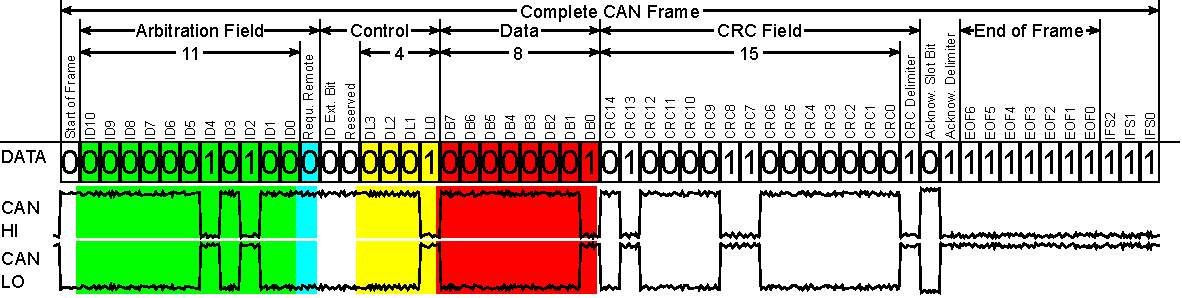
\includegraphics[width=0.4\textwidth]{can_frame.pdf}
  \caption{CAN Frame without bit stuffing}
  \label{fig:can_frame}
\end{figure}

Can was the first industrial protocol for vehicles, and CAN is used for nearly
all systems of a vehicle, except for the comfort system which require higher
bandwidth than CAN provides.

\subsection{LIN}
LIN is a class A, half duplex, master initiated network type. It provides a low
cost network capable of interfacing up to 16 separate slave units. LIN is
typically used to create small local networks of sensors, which contribute data
to a master ECU who in turn communicates on a vehicle wide CAN bus
\autocite{lukasiewycz_system_2013}.  This reduces the cost and complexity since
LIN can be implemented on a single wire, with hardware as simple as a UART
\autocite{std_lin}.  

LIN to support the constraint of trivial hardware, LIN does not implement
a priority mechanism at the physical level, and instead relies on a master-slave
mechanism. In LIN, all communicate is initiated from the master. The master then
ensures that the latency requirements of individual nodes are met. While this is
not as scalable as CAN's priority mechanism, LIN's limited size makes it very
useful for smart sensors to publish data.

\begin{figure}
  \centering
  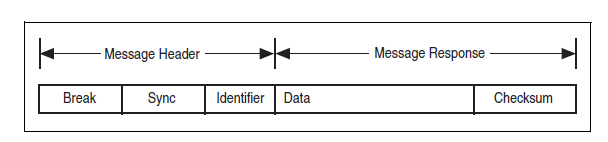
\includegraphics[width=0.4\textwidth]{LIN_frame.png}
  \caption{LIN frame}
  \label{fig:lin_frame}
\end{figure}

\subsection{FlexRay}
FlexRay is a Class D, full duplex self initiated, network type. It provides very high performance up to 10
Mbps while retaining a strong transmission error correction scheme.  FlexRay
supports both optical and electrical transport on the physical layer.  To
address availability, FlexRay divides transmission into major frames. Each major
frame is divided into two minor frames, a static frame and a dynamic frame. The
static frame implements a master schedule system reserving fixed periods of
time to fixed ECUs.  The dynamic phase allows for event triggered messages
similar to CAN \autocite{luo_research_2008}.  

\begin{figure}
  \centering
  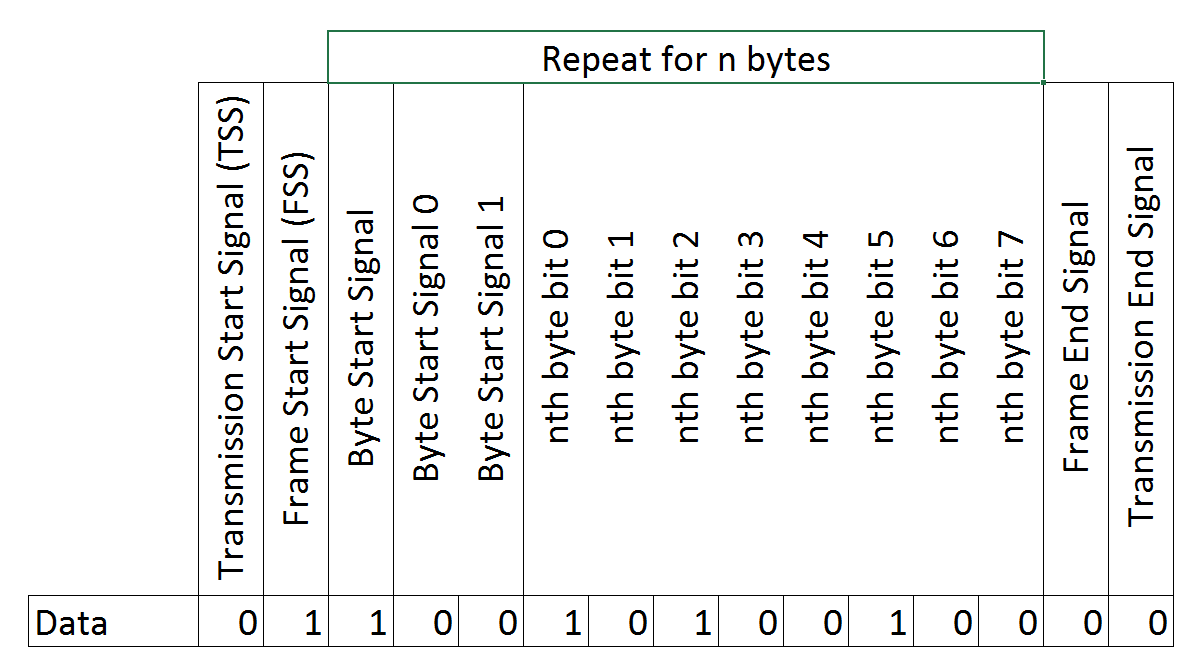
\includegraphics[width=0.4\textwidth]{Flexray.PNG}
  \caption{FlexRay frame}
  \label{fig:flexray_frame}
\end{figure}

For data integrity FlexRay provides a 24bit CRC. FlexRay supports both star
networks for highest performance,  or multi-drop media for reduced cost. FlexRay
support dual channels each operating at up to 10 Mb/s. This adds extra
reliability. FlexRay pushes strict system requirements on maximum allowable clock
drift of 0.15\%. While this accuracy cannot be achieved with a standard
microcontroller RC oscillator, a quartz crystal oscillator can provide this
level of precision quite easily \autocite{_crystal_2014}. Cheng-lin shows how
FlexRay's reliability is independent of bus loading where can's reliability
degrades as the bus becomes loaded \autocite{cheng-lin_real-time_2010}.  In CAN
lower priority messages are held off while higher priority messages are
transfered summarized in Figure~\ref{fig:can_vs_flexray_reliability}. Using
a Poisson error model, Cheng models the delay of low priority messages as
a function of the bus load. Intuitively this makes sense, CAN messages are event
triggered, and both the software layers, and hardware layers route highest
priority messages first. Then if an important, but not quite the highest
priority
message is sitting in an ECU queue, it can wait a long period of time until it
has an opportunity to send the message.
Figure~\ref{fig:can_vs_flexray_reliability} shows that this error
exponentially approaches 100\% probability of failure, eventually failing at
bus load of about 90\%. FlexRay however remains constant within this error
model using two mechanisms. Firstly the static domain will route all priority messages according
to the defined schedule. This is the benefit of Time triggered networks,
something that \emph{could} be done with CAN, but wasn't part of the original
intent. Secondly, FlexRay provides redundancy in two methods. Firstly FlexRay
defines a dual channel redundancy allowing a failed bus to send data over a back
channel. For the highest level of reliability however, FlexRay supports Dual
message, Dual channel which sends duplicate data over the redundant channel,
hence sending all messages twice.  This is the highest level of reliability and
according to Cheng results in a total probability of failure of $7.374 \times
10^{-50}$.

\begin{figure}
  \centering
  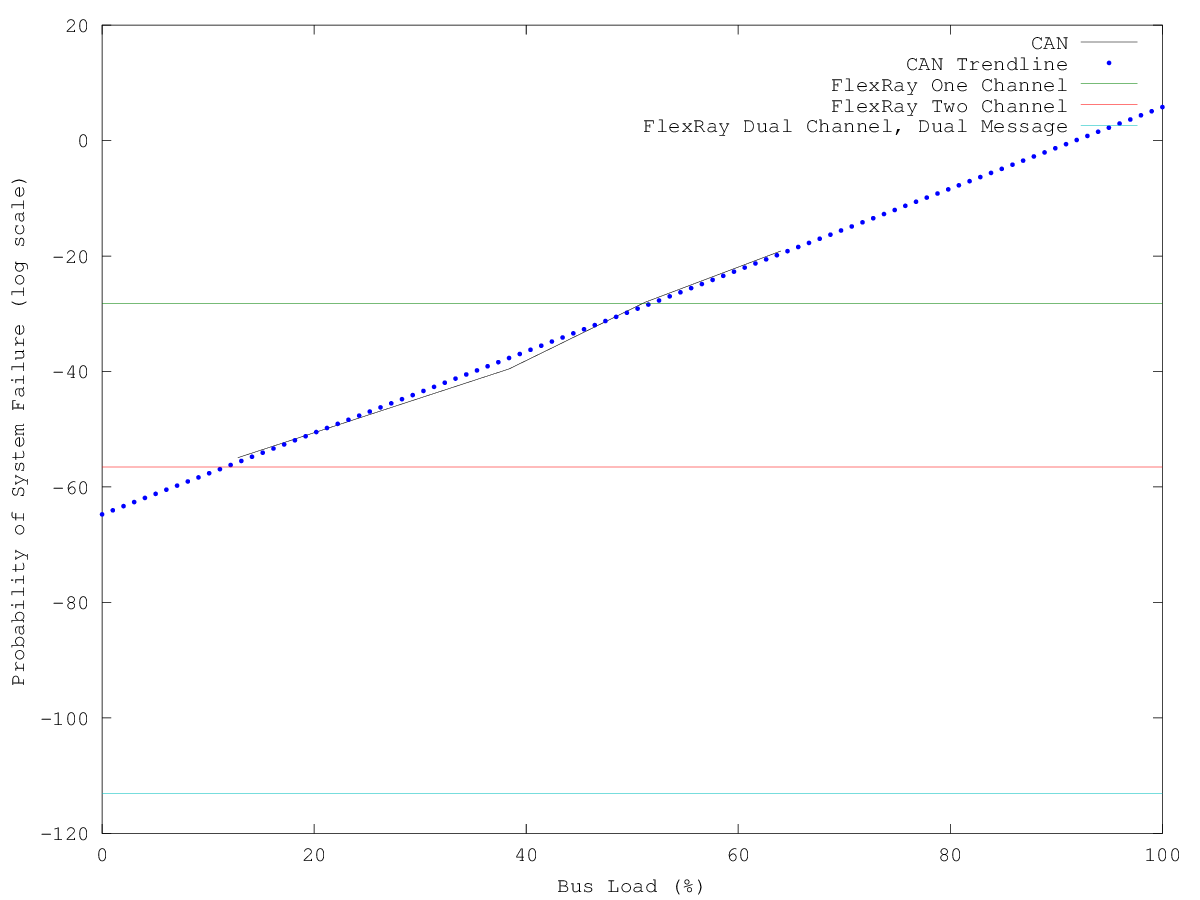
\includegraphics[width=0.4\textwidth]{FlexRaySystemReliability.png}
  \caption{CAN vs FlexRay Reliability}
  \label{fig:can_vs_flexray_reliability}
\end{figure}


\section{Messaging Schemes}
We've seen how the physical layer of CAN provides a priority scheme, but its
reliability is still susceptible to bus load factors. FlexRay's physical layer
however incorporates a two phase major frame to support both priority and time
based messages, additionally providing dual channel and redundant messaging
resulting in a strongly reliable protocol.  However by stepping up a layer from
the physical, we can improve the reliability of CAN bu incorporating some of
FlexRay's time trigger concepts. This is the principle between message schemes.
At a layer above the physical layer, we can provide additional guarantees to
provide a more reliable channel. Similar to how TCP provides an in-order
guaranteed deliver over IP, WE can provide guaranteed access for CAN.

Each of the network types we've looked at are single media, multiple access
networks.  All ECUs, share a single set of wires to communicate to each other.
Ethernet is also such a configuration. However Ethernet's start of transmission
scheme is in start contract to industrial protocols presented here. Ethernet has
a randomized backoff scheme which manifest a variable network latency scheme.
If a device is a very loud talker, it can push out all other communication
creating a classic denial of service. In a vehicle bus, denial of service, i.e.
the steering wheel cannot contact the power steering unit as in a steer-by-wire
system. Such an event renders the vehicle an uncontrollable missile. But where Ethernet has variable latency
due to its randomized start of transmission scheme, industrial protocols have
two major schemes time triggered, and event triggered messaging for dealing with denial of service, and define a fixed
latency. 

\subsection{Time Triggered Messages}
\label{sec:time_trigger}
Time triggered message schemes send data at a rated defined by a network
``master schedule''. This is essentially time division multiplexing the
communication channel. The upside to time triggered messaging is the simplify
of analysis. When all messages are defined for bounded windows of transmission,
it is explicitly known what all message latencies are.  The downside is
composability. Vehicle manufactures tend to build vehicle systems over time,
making small improvements and composing new functions reusing smaller functions
which already exist. Since the ``master schedule'', is truly a single document
describing all traffic, adding a new ECU to the network requires the entire
schedule to be redesigned and evaluated. 

Time triggered messaging is primarily used in fail-safe systems such as steering
and braking. BMW's steer-by-wire systems use FlexRay for very high speed
communication, between the steering wheel, and the steering actuators. The
steering wheel sends it's current angle, and velocity periodically to the
actuator. If the actuator doesn't receive a message from the steering wheel on
the scheduled time, it can perform some error mechanism to protect the vehicle
from a potentially failed steering wheel.  Braking is a similar design allowing
the vehicle to fail safely if communication channels are faulty. 

\subsection{Event Triggered Messages}
Event triggered schemes preserve bandwidth over time triggered schemes since
ECUs are not sending repeat messages at defined rates. This allows lower speed
buses such as Low speed CAN (125Kbps) to more efficiently use the
limited performance. This however can make the latency more difficult to reason
about. If the message schema does not support priority, then its possible for
lower priority messages to flood the bus, and prevent higher priority messages
from reaching the destination before the deadline. 

\section{System Architecture}

Now with various message schemes, over various transport, how are these pulled
together to a consistent system architecture.
Figure~\ref{fig:heterogenous_network} shows a typical breakdown of networks
according to the various functions within a vehicle. Initially, requirements are
broken down into the primary categories of vehicle networks.  Infotainment
systems include connectivity, GPS, music, and entertainment systems. These
systems are bandwidth heavy, but do not require high safety, for these MOST
(Media Oriented Service Transport) is typically used providing up to 12.5 Mbps.
Next comes the dash, and instrument panels. Typically these don't require high
bandwidth, but reliability and safety is paramount, this is a fit for time
triggered CAN.  Next comes electronic door locks, mirror adjustments, and other
simple control mechanisms. For these LIN is a great fit, since they require low
safety, and low speed.  Lastly, Engine, and transmission data. Drive by wire,
and electronic shifting. 
\begin{figure}
  \centering
  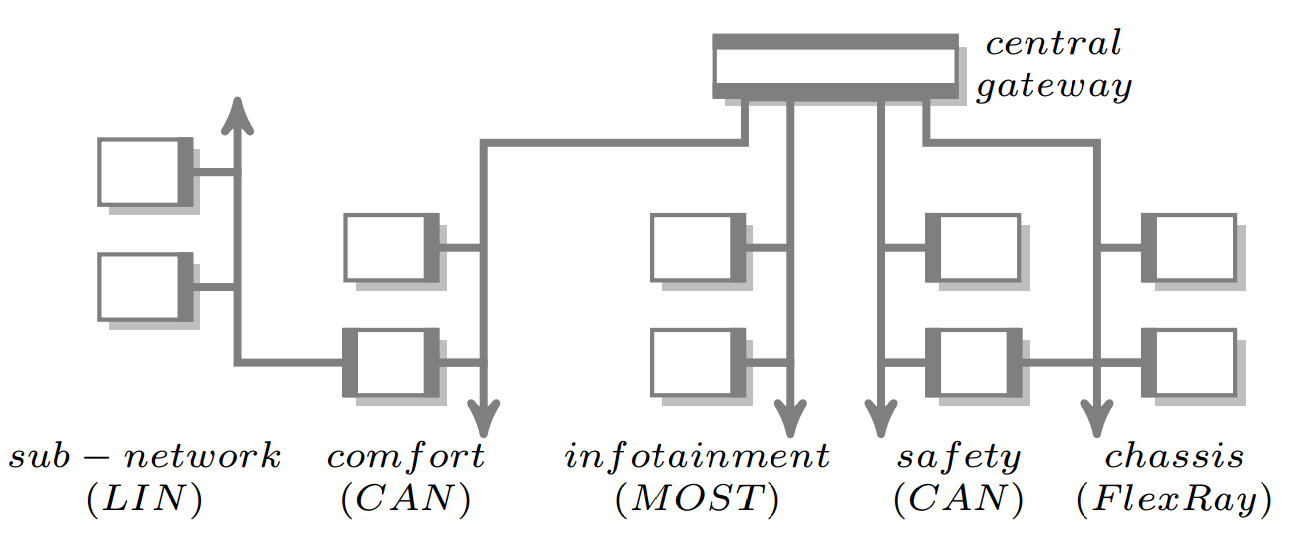
\includegraphics[width=0.4\textwidth]{network_topography.png}
  \caption{Heterogeneous Vehicle Network \autocite{lukasiewycz_system_2013}}
  \label{fig:heterogenous_network}
\end{figure}

Engines have grown exponentially in the amount of data they require to operate
properly. Currently Mercedes vehicles are using up to 70 ECUs
\autocite{guo_integrated_2009}.

\section{Conclusion}
Vehicle electronic are trending toward higher connectivity, higher security, and
greater integration within the vehicle as well as new out of vehicle systems.
These trends are already pushing the performance limits of its backbone protocol
CAN, and while MOST provides a higher bandwidth link, it cannot complete with
the safety offered by FlexRay.

As our vehicles are increasingly connect

It is an exciting time to see what advanced will be
made in the realm of vehicle protocols to meet this growing bandwidth bottleneck,
but maintain the critical safety specifications which keeps us blissfully unaware
of the mountain of software that make our cars function. 

\printbibliography

\end{document}
